\documentclass[12pt]{article}

\usepackage[margin=1in]{geometry}
\usepackage{setspace}
\usepackage{mathptmx}
\usepackage[T1]{fontenc}
\usepackage[utf8]{inputenc}
\usepackage{graphicx}
\usepackage{float}
\usepackage{textcomp}
\usepackage{amsmath}
\usepackage{natbib}
\usepackage[hyphens]{url}
\usepackage{xurl}
\usepackage[hidelinks]{hyperref}
\usepackage{booktabs}
\usepackage{tikz}
\usetikzlibrary{arrows.meta, positioning}
\usepackage{pgfplots}
\pgfplotsset{compat=1.18}

\doublespacing
\setlength{\parindent}{0pt}
\setlength{\parskip}{0.5em}

\begin{document}

\title{Group Assignment 6: Economic Analysis of Japanese Negative Interest Rates\\[0.5em]}
\author{Logan Rechin, Joe White\\ECO 442}
\date{April 22, 2026}
\maketitle

In March 2024, the Bank of Japan ended its negative interest rate policy and raised interest rates for the first time in seventeen years \citep{boj2024statement}. The decision moved Japan's short-term policy rate from negative territory to a target range of 0 to 0.1 percent. In a simple asset-market model, a higher domestic interest rate should make domestic assets more attractive and lead to an appreciation of the domestic currency. Instead, the yen weakened against the U.S. dollar after the announcement \citep{reuters2024yen}. This leads to our main question: why did the yen depreciate even though the Bank of Japan raised interest rates?

Negative interest rates do not mean that cash automatically loses value. Instead, they mean that commercial banks can be charged for holding certain reserve balances at the central bank. In Japan, the Bank of Japan applied a rate of -0.1 percent to part of the current account balances held by financial institutions \citep{boj2024minutes}. For example, if a bank held reserves subject to the negative rate, it would pay the Bank of Japan to keep those reserves there instead of earning interest on them. The purpose of the policy was to encourage lending, lower broader interest rates, and help move inflation toward the Bank of Japan's 2 percent target.

There are limitations to negative interest rates. If rates become too negative, banks may become less profitable, and households or firms may prefer to hold cash instead of deposits. This is part of why negative interest rate policy is seen as unusual. Japan used it because the country had struggled for years with low inflation, weak demand, and slow growth. The policy was part of an attempt to stimulate the economy and move inflation closer to the central bank's target.

This helps explain why the March 2024 decision mattered. The Bank of Japan was ending a policy regime that had been associated with Japan's long fight against deflation. Because of that, the decision initially seemed like it should strengthen the yen. However, the actual market reaction was different.

The asset model and interest rate parity give a framework for understanding this event. Exchange rates are forward-looking asset prices because investors compare the expected return on domestic deposits with the expected return on foreign deposits. In the simplest version of the model, a Japanese interest rate increase should strengthen the yen because it raises the expected return on yen assets. This should increase demand for yen assets and cause the yen to appreciate. However, this prediction only holds cleanly when foreign interest rates and expected future exchange rates are held constant. In March 2024, those assumptions were not realistic. U.S. interest rates remained much higher than Japanese interest rates, and the Bank of Japan's announcement did not convince markets that Japan was beginning tightened monetary policy.

The first reason the yen did not appreciate is that the interest rate increase was small. The Bank of Japan ended its negative interest rate policy, but the new target rate was only 0 to 0.1 percent \citep{boj2024statement}. By comparison, the Federal Reserve kept the target range for the federal funds rate at 5.25 to 5.50 percent at its March 2024 meeting \citep{fed2024statement}. Therefore, even after the Bank of Japan's historic announcement, the U.S.-Japan short-term interest rate differential remained large. The symbolism of ending negative rates was much larger than the actual change in relative returns. Table \ref{tab:policy_rates} summarizes this interest rate comparison.

The second reason is that the announcement did not strongly change expectations about future Japanese monetary policy. The Bank of Japan stated that it would continue bond purchases and that financial conditions would likely be maintained for the time being \citep{boj2024statement}. This language mattered because it suggested that the end of negative rates was not the beginning of monetary tightening. Reuters also described the decision as widely anticipated \citep{reuters2024yen}, meaning that markets had already expected the policy change before the official announcement. Since exchange rates respond to new information, an expected rate increase would not necessarily cause the yen to appreciate on the announcement date.

Figure \ref{fig:yen_dollar} shows what happened to the yen-dollar exchange rate before and after the policy announcement. Because the exchange rate is measured as yen per dollar, an increase means that the yen is depreciating. If financial markets had viewed the Bank of Japan's decision as a strong monetary tightening, we would expect the yen to appreciate after the announcement. Instead, the figure shows that the yen remained weak around the event window.

The U.S. dollar is still important in this case because the United States is Japan's largest export market and the dollar is the main international reserve currency. However, the yen-dollar exchange rate is not the only relevant exchange rate for Japan. Japan's main export partners in 2023 were the United States, China, South Korea, Hong Kong, and Thailand, while its main import partners included China, the United States, Australia, the United Arab Emirates, and Saudi Arabia \citep{santander2024japantrade}. For that reason, the yen's movement against other major currencies should also be considered. If the yen weakened broadly, then the explanation is more likely about Japanese monetary policy and global investor expectations rather than only a U.S.-Japan issue.

The key point is that investors care about relative expected returns, not just whether one central bank raises rates. Even after the Bank of Japan ended negative interest rates, yen assets still offered much lower short-term returns than dollar assets. In addition, the Bank of Japan did not signal that it would quickly continue raising rates. Its statement suggested that financial conditions would remain stable. If investors expected Japan to remain cautious while the United States continued to offer much higher returns, then dollar assets could still look more attractive than yen assets. In that case, the yen could weaken even after a Japanese rate increase.

This interpretation fits the short-run asset model. The March 2024 announcement affected financial markets immediately because investors could quickly adjust their holdings of yen and dollar assets. By contrast, changes in goods markets work more slowly because prices, exports, and imports do not fully adjust overnight. Therefore, the immediate yen depreciation after the announcement is best understood as an asset-market reaction to expected returns and future policy, not as a direct response to changes in Japanese trade flows.

Overall, the yen weakened after the Bank of Japan ended negative interest rates because the announcement was historic but not very contractionary. The policy rate moved only to 0 to 0.1 percent, while U.S. rates remained above 5 percent. In addition, the decision was widely expected and the Bank of Japan signaled that financial conditions would remain accommodative. The event therefore shows that exchange rates respond not only to whether a central bank raises rates, but also to the size of the increase, the foreign interest rate comparison, and expectations about future policy.

\begin{thebibliography}{9}

\bibitem[Bank of Japan(2024a)]{boj2024statement}
Bank of Japan. 2024a. ``Changes in the Monetary Policy Framework.''
March 19, 2024.
\url{https://www.boj.or.jp/en/mopo/mpmdeci/mpr_2024/k240319a.pdf}

\bibitem[Bank of Japan(2024b)]{boj2024minutes}
Bank of Japan. 2024b. ``Minutes of the Monetary Policy Meeting on March 18 and 19, 2024.''
\url{https://www.boj.or.jp/en/mopo/mpmsche_minu/minu_2024/g240319.htm}

\bibitem[Board of Governors of the Federal Reserve System(2024)]{fed2024statement}
Board of Governors of the Federal Reserve System. 2024. ``Federal Reserve Issues FOMC Statement.''
March 20, 2024.
\url{https://www.federalreserve.gov/newsevents/pressreleases/monetary20240320a.htm}

\bibitem[Reuters(2024)]{reuters2024yen}
Reuters. 2024. ``Yen Holds Nerve as BOJ Decision Looms, Dollar Resurgent.''
March 19, 2024.
\url{https://www.reuters.com/markets/currencies/yen-holds-nerve-boj-decision-looms-dollar-resurgent-2024-03-19/}

\bibitem[Federal Reserve Bank of St. Louis(2026)]{fred_yen}
Federal Reserve Bank of St. Louis. 2026. ``Japanese Yen to U.S. Dollar Spot Exchange Rate [DEXJPUS].''
FRED, April 22, 2026.
\url{https://fred.stlouisfed.org/series/DEXJPUS}

\bibitem[Santander Trade(2024)]{santander2024japantrade}
Santander Trade. 2024. ``Japanese Foreign Trade in Figures.''
\url{https://santandertrade.com/en/portal/analyse-markets/japan/foreign-trade-in-figures}

\end{thebibliography}

\newpage
\section*{Figures}

\begin{figure}[h!]
    \centering
    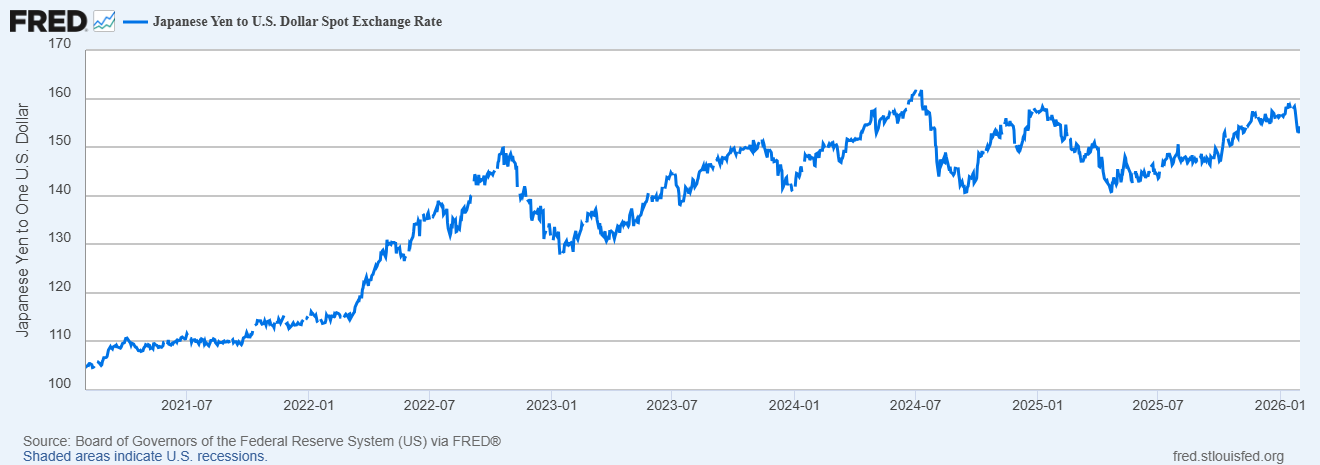
\includegraphics[width=0.82\textwidth]{fredgraph.png}
    \caption{Japanese yen per U.S. dollar around the March 19, 2024 Bank of Japan announcement}
    \label{fig:yen_dollar}
    \begin{minipage}{0.9\textwidth}
    \begin{singlespace}
    \footnotesize
     Source: FRED, Japanese Yen to U.S. Dollar Spot Exchange Rate.
    \end{singlespace}
    \end{minipage}
\end{figure}

\vspace{2em}

\begin{table}[h!]
\centering
\caption{Short-term policy rates around the March 2024 BOJ announcement}
\label{tab:policy_rates}
\begin{tabular}{lcc}
\toprule
Country & Before March 2024 & After March 2024 \\
\midrule
Japan & -0.1\% & 0 to 0.1\% \\
United States & 5.25 to 5.50\% & 5.25 to 5.50\% \\
\bottomrule
\end{tabular}

\vspace{0.75em}
\begin{minipage}{0.9\textwidth}
\begin{singlespace}
\footnotesize
Sources: Bank of Japan and Federal Reserve.
\end{singlespace}
\end{minipage}
\end{table}

\end{document}